\subsection{Closed-loop testing of pacemaker}
\label{closedloop}

\begin{figure}[t]
\centering
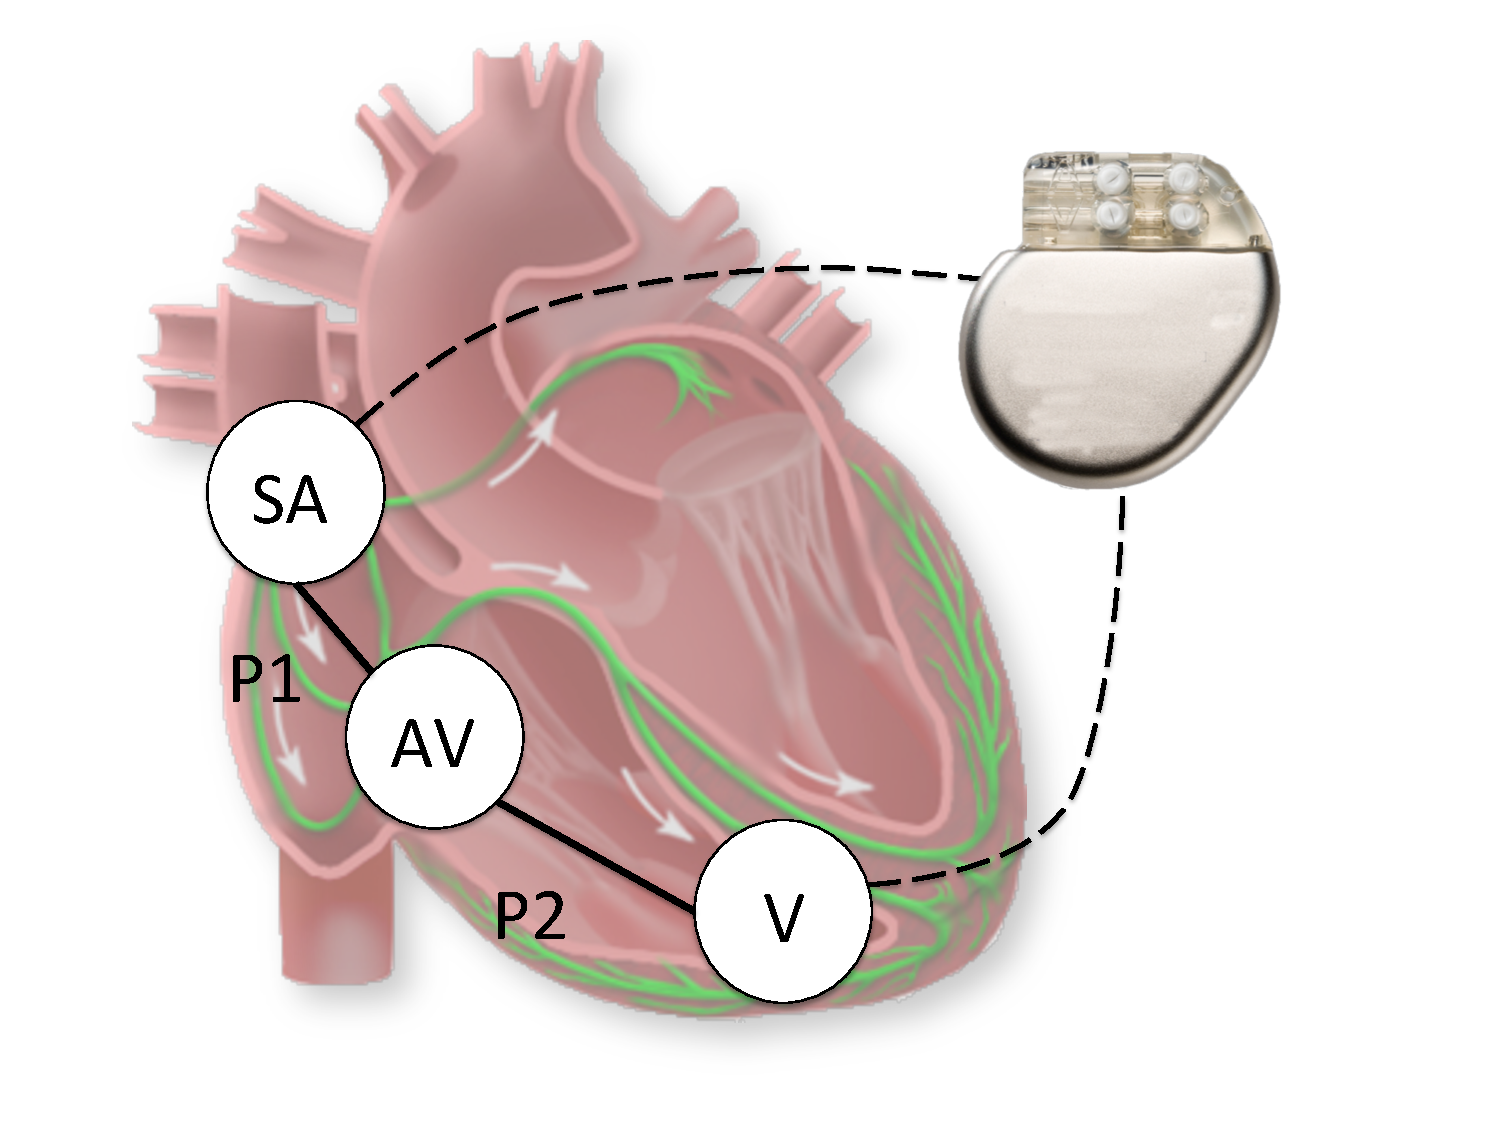
\includegraphics[scale=0.2]{figures/nodesandPM}
\caption{Portion of the VHM: the conduction paths P1 and P2 connect the SA node to the ventricle V via the AV node (solid line). The pacemaker induces a second, `virtual', pathway (dashed line).}
\label{fig:nodesandPM}
\vspace{-.5cm}
\end{figure}

\textbf{Closed-loop setup}.
The closed-loop setup is shown in Fig.~\ref{fig:reqGuidedTesting}.
The VHM and pacemaker are connected in the same way as a real heart and pacemaker would be connected.
Thus, the inputs to the pacemaker are automatically generated by the VHM as atrial and ventricular sensing events (AS and VS), and don't need to be pre-programmed by the validation engineer as they would be in open-loop testing. 
The VHM, in turn, is stimulated by the pacemaker's Atrial and Ventricular Pacing events (AP and VP).
In addition, the tester is connected at the PVC `inputs' to the heart.
That is, the tester provides waveforms that mimic  PVC events as will be explained below.
The tester can read all required signals from the VHM.
In our experiments, it reads five waveforms: the depolarization events at SA node, AV node, and ventricle (SA, NA and V), and the conduction state of paths P1 and P2 connecting them. (See Fig.~\ref{fig:nodesandPM}.)
It also reads the AP and VP events from the pacemaker.

\textbf{Tester-controlled inputs}.
In our setup, the testing algorithm will generate Premature Ventricular Complex (PVC) waveforms to mimic the abnormal depolarizations of the ventricles that occur in the human heart, and can fool the pacemaker sensing. 
A \emph{test} is then defined as a PVC waveform of a pre-determined duration $T$ ms.
These are used by the tester to try and cause the closed loop to manifest unsafe or undesirable heart conditions.
The constraint on the waveforms generated by the tester is that there should be at least 400ms between consecutive PVC impulses.
More generally, the tester can also generate Premature Atrial Contraction events and vary the closed loop parameters within their physiological range.

\textbf{The tester}.
The tester itself is a requirements-guided automatic test generation algorithm, whose theory is given in \cite{AbbasFSIG13tecs}, and we review it here briefly.
This testing algorithm has been implemented in the tool S-Taliro \cite{AnnapureddyLFS11tacas}, and has been used in other medical applications like the analysis of insulin infusion pumps schedules \cite{SankaranarayananF2012cmsb}.
The operation of the tester is as follows: we provide S-Taliro with a specification that the pacemaker+heart closed loop must satisfy,
e.g., ``there should be a minimum delay of 500ms between VP events''.
S-Taliro iteratively tries to find a test (i.e., a PVC waveform or pre-determined duration) such that the resulting closed loop behavior \emph{violates} the specification.
S-Taliro does this by iterating the following process: it generates a test, and observes the output waveform from the closed loop and calculates the \emph{the degree} to which it satisfies the specification or not.
This degree is then used to choose the next test to apply. 
It can be shown that if the system can exhibit a behavior that violates the specification, then this iterative process converges to a test that will provoke this incorrect behavior \cite{AbbasF_HybridSA12}. 
This test then serves as evidence that the pacemaker+heart loop can exhibit undesired behavior that violates the specification.
The pacemaker's designer can then replay this test to see where things went wrong, and whether the pacemaker needs to be adjusted accordingly.

\textbf{Advantages over open-loop testing}.
The advantages of the proposed requirements-guided closed-loop testing approach over directed open-loop testing are summarized in Table \ref{table:CLoverOL}, and discussed here:
\begin{table*}
	\centering
	\caption{Comparison between open-loop and proposed closed-loop testing.}
	\begin{tabular}{|l|l|l|}
	\hline                       & Open-Loop    & Requirements-Guided Closed-Loop 
	\\ 
	\hline Choice of pacemaker input traces  
	                & Manual and recorded traces. Might miss interesting behavior, &  Automatic and provided by the VHM,
	\\ 
					& or include irrelevant behavior. &  so only relevant input traces are used.
	\\
	\hline Criterion of correctness    & Only pacemaker behavior & The heart and pacemakers's joint behavior, so 
	\\
	                &                  & physiological effects of pacemaker actions
	\\
	                &                  &  can be used to determine correctness.                   
	\\ 
	\hline Choice of tests & Tests = input traces to pacemaker.  & Tests = traces of external disturbances, 
	\\
	                & Manually chosen.  & like PVC and PAC. Automatically selected by S-Taliro.
	\\
	\hline 
\end{tabular}
\label{table:CLoverOL}
\end{table*}

\begin{figure}[t]
\centering
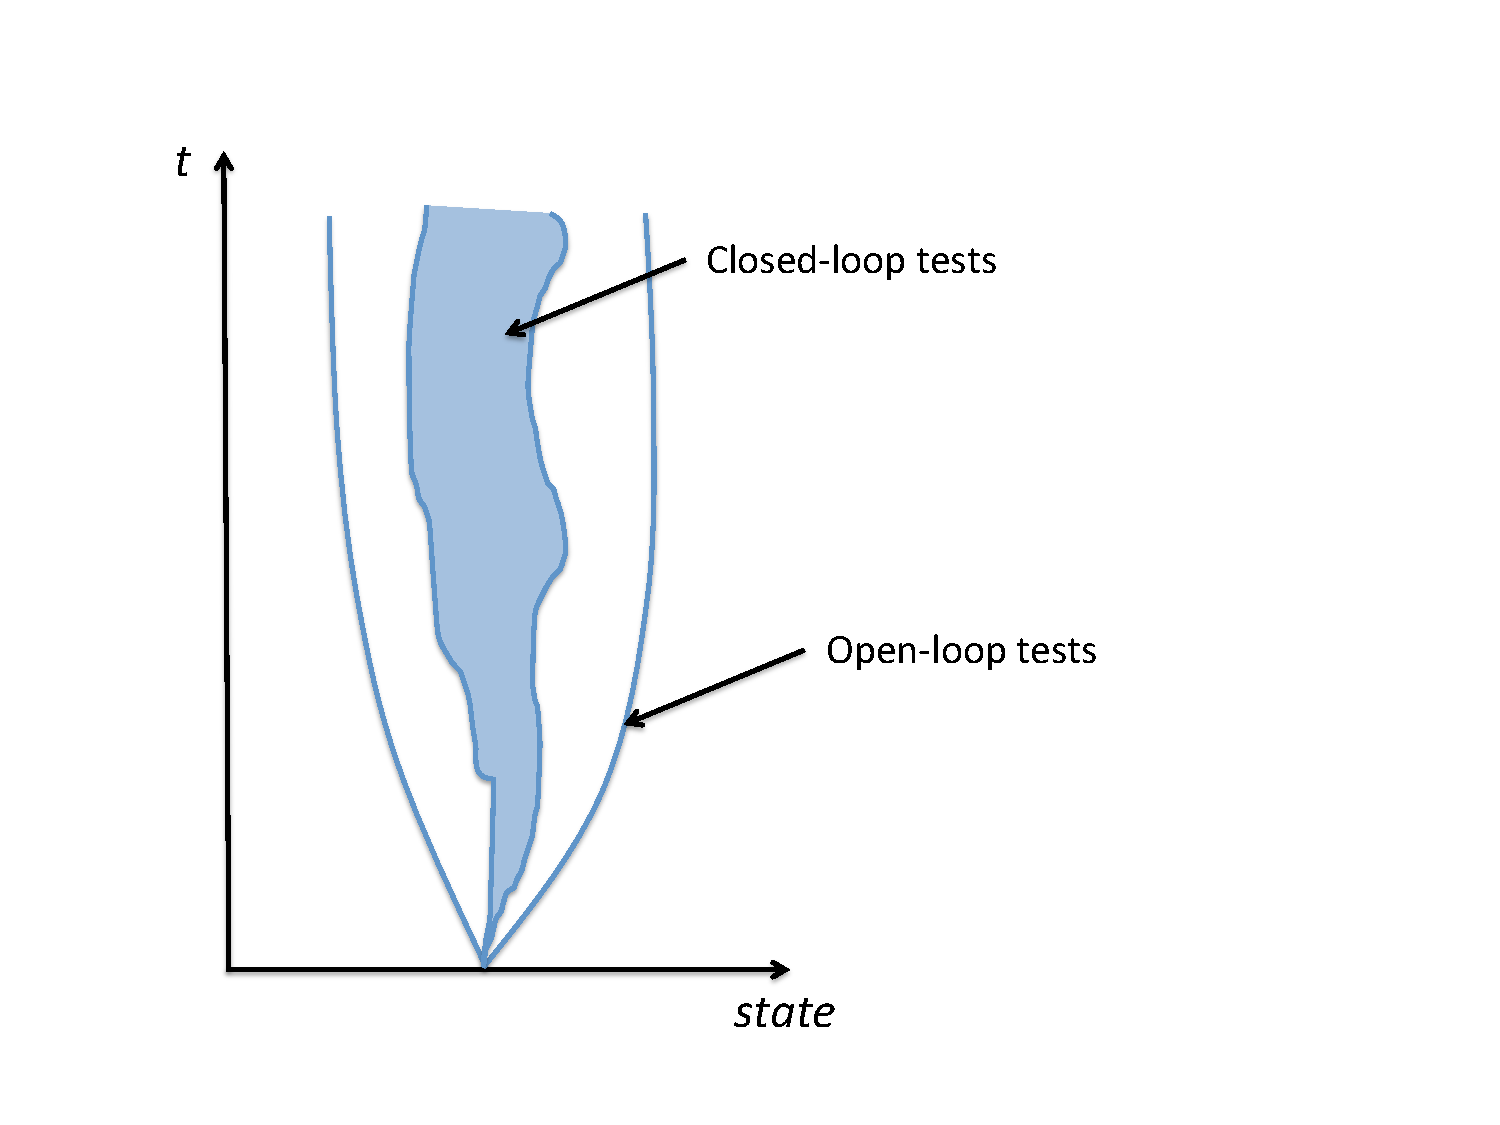
\includegraphics[scale=0.3]{figures/cone}
\caption{The space of closed-loop inputs to the pacemaker is constrained by the VHM and is thus smaller than the open-loop space.}
\label{fig:cone}
\vspace{-.2cm}
\end{figure}

\begin{itemize}
	\item Choice of inputs: because a heart model provides the input traces to the pacemaker, we know that only relevant test cases will be generated. 
	That is, only traces that the pacemaker may actually see during live operation are fed to it during testing. 
	\footnote{Of course, this ultimately depends on the quality of the VHM.}
	Compare this to open-loop testing where nothing constrains the inputs, as illustrated in Fig.~\ref{fig:cone}.
	It is difficult if not impossible to reason a priori about how the heart will constrain the pacemaker's inputs, especially for \emph{deep} behaviors that take a long time to occur.	
	Moreover, because the tester produces the tests systematically, we are guaranteed to find violating behavior if it exists.
	\item Criterion of correctness: because we have a VHM, we can express correctness \emph{as a property of the heart's behavior}, and not of the pacemaker alone. 
	Thus we can evaluate what truly matters: is the heart (as modeled by the VHM) displaying unsafe or undesirable behavior?
\end{itemize}

%\textbf{Choice of specifications to test}.
%Because the heart's behavior is complex and varies depending on its physiological structure and history, it is not always easy to describe succinctly what is `unsafe' and what is `undesirable'.
%Both categories vary depending on what we know (and what we discover) about the heart conditions being modeled.

\textbf{Interpretation of testing results}.
It must be stressed that the interpretation of closed-loop testing results depends on the specific violating behaviors that are found.
Some will be determined to be bugs in the pacemaker (or VHM). 
Others will be determined to be undesirable but unavoidable behaviors, and we show such a case in Section \ref{experiments}.
%This is because specifying `safe' behavior can be difficult for something as complex as the heart.
